\section{BLEEX}
\label{exo:bleex}
\begin{refsection}[exos/bleex.bib]

keywords: sensitivity amplification; strength augmentation.\\

The Berkeley lower extremity exoskeleton (BLEEX) is an anthropomorphic, powered exoskeleton designed for human strength augmentation.  It is described as the first field-operational robotic system to allow its operator to carry significant loads over unstructured terrain without external power \cite{bleex_design_2006}.

\begin{figure}[ht]
  \centering
  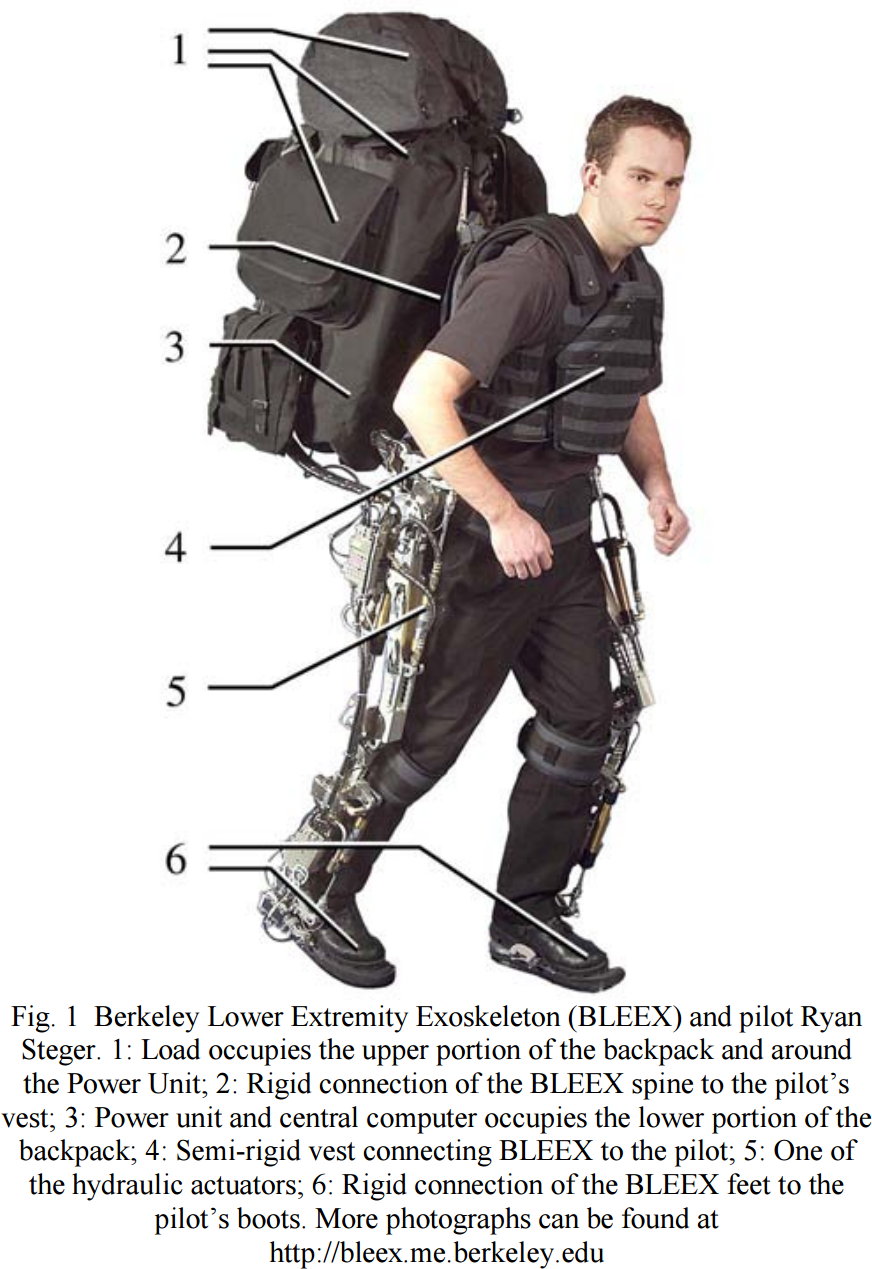
\includegraphics[width=3.5in]{exos/figs/bleex_exo.png}
\end{figure}

The BLEEX system includes two 7 DOF, three-segment legs with thigh, shank, and foot links, on-board power supply, and a backpack-like frame.  The human wearer is rigidly connected at the feet and torso such that the frame shelters the user by transferring load forces to the ground.  The leg segments are connected by rotational joints including 3 DOF (2 actuated) at the hip, 1 DOF (actuated) at each knee, and 3 DOF (1 actuated f/e in sagittal 
plane; 2 passive) at the ankles.  Joint angles, torque, and power requirements are determined from human motion analysis based on a 75-kg human walking on flat ground at roughly 1.3 m/s (the average military male's maximum reported joint limits are also used to derive joint range of motion targets).  During design, joint motion was intended to be slightly less than the maximum human range of motion for safety; however, some joint ranges had to be reduced to avoid singularities.
% Ideally, joint motion would provide the maximum human range of motion for safety

Due to its high power to weight ratio (twice that of electric motors), BLEEX uses a hydraulic actuation system.  An on-board internal combustion engine provides both electric and hydraulic power.  The joints are driven by commercial small bore (2cm) dual action hydraulic actuators operating at 6.9 MPa. Though the operating pressure is relatively low, the hydraulic actuation system exhibits significant pressures losses across servo valves when less pressure is required than this system pressure.  Table~\ref{tab:bleex_joints} provides details regarding the range of motion and torque capabilities of BLEEX's joints.  As reported in \cite{bleex_design_2006}, BLEEX requires 1,143 W for walking relative to 165 W for human walking (14\% efficient compared to a human of the same size).  Altogether the suit needs 2.27 kW of hydraulic power and 220 W of electric power to accommodate climbing (540 W) and remaining electrical loads including 240 W to power the second stages on servo vales.

%
\begin{table}
\centering
\begin{tabular}{|l|*{3}{c|}}  % repeats {c|} 6 times
\hline
& BLEEX & human max & BLEEX \\
& ROM & torque \& power & max torque \\ \hline
Ankle flexion / extension & $\pm 45^\circ$ & $-120$ N-m; 250 W & $-200 / 155$ N-m\\ \hline
Ankle abduction / adduction & $\pm 20^\circ$ & N/A & N/A \\ \hline
Knee flexion & $121^\circ$ & $-35 / 60$ N-m; $-150 / 50$ W & $-100 / 140$ N-m \\ \hline
Hip flexion / extension & $\pm 121^\circ / 10^\circ$ & $-80 / 60$ N-m; $-60 / 115$ W & $-150 / 130$ N-m \\ \hline
Hip abduction / adduction & $\pm 16^\circ$ & N/A & N/A\\ \hline
total rotation external & $35^\circ$ & N/A & N/A \\ \hline
total rotation internal & $35^\circ$ & N/A & N/A \\ \hline
\end{tabular}
\caption{BLEEX joint range of motion (ROM) is near anthropomorphic.  The max torques are designed to meet the torque / power requirements of similarly sized human walking at 1.3 m/s \cite{bleex_design_2006}.}\label{tab:bleex_joints}
\end{table}
%

\subsubsection{Control}

The BLEEX team has successfully implemented both sensitivity amplification \cite{sesitivityAmpPaper2005} and a hybrid assitive control scheme \cite{bleex_hybrid_control_2006} that switches (based on gait phase) between sensitivity amplification and a position control regulating desired torque. This section focuses on sensitivity amplification, as the hybrid assitive strategy did not perform as well in walking trials.

\begin{figure}[ht]
  \centering
  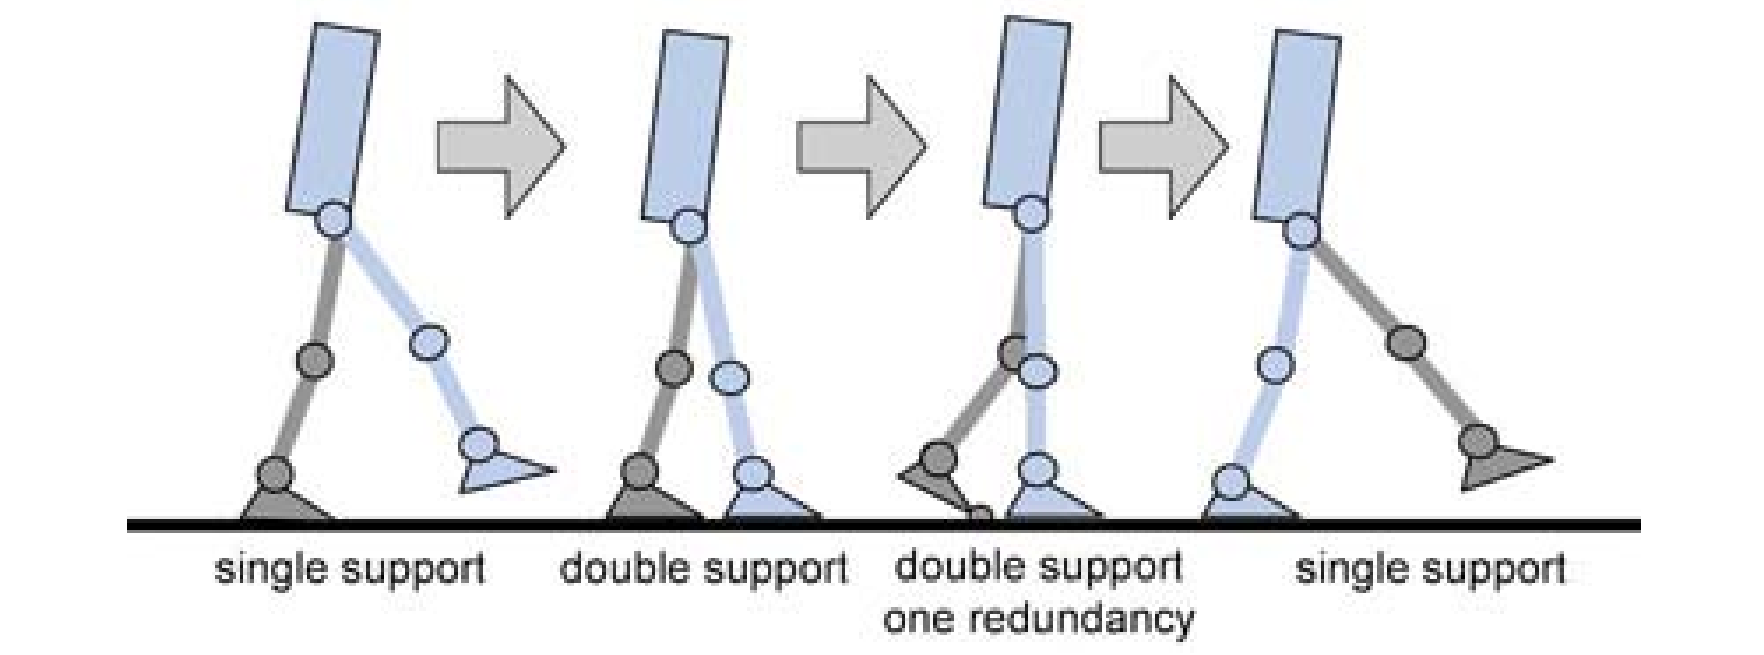
\includegraphics[width=3.5in]{exos/figs/bleex_support_phases.png}
\end{figure}

In its sensitivity amplification implementation, BLEEX controllers attempt to minimize interaction forces between the human pilot and the exoskeleton. However, the BLEEX team makes a point to avoid direct measurements of the interaction force between the human and the exoskeleton suit.  They highlight difficulties in properly outfitting humans with necessary sensing equipment and challenges in modeling the interaction between the human and exoskeleton (e.g., non-rigid, non-fixed contact points).  Instead, the team develops controllers based on an inverse dynamic model (in the saggital plane) of only the exoskeleton.  

\begin{figure}[ht]
  \centering
  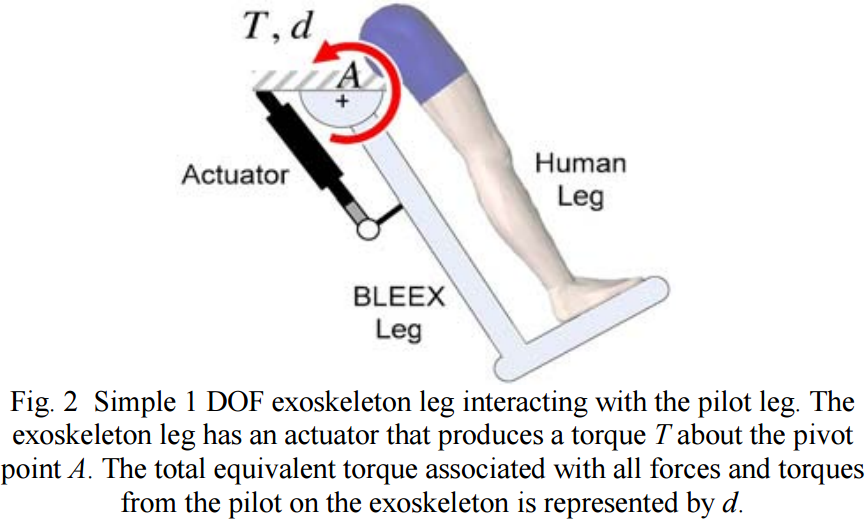
\includegraphics[width=3.5in]{exos/figs/bleex_1dof_ex.png}
\end{figure}

The BLEEX sensitivity amplification control strategy models the torque applied by the human pilot on the exoskeleton as $d$ (assuming no outside disturbances).   Neglecting gravity, the exokeleton angular velocity is modeled as 
\[v = G r + S d ,\] 
where $G$ is the transfer function from actuator inputs ($G$ is the exoskeleton's dynamics), $r$ is the actuator input, and $S$ is the sensitivity or transfer function from human torque to exokeleton angular velocity. 

\begin{figure}[ht]
  \centering
  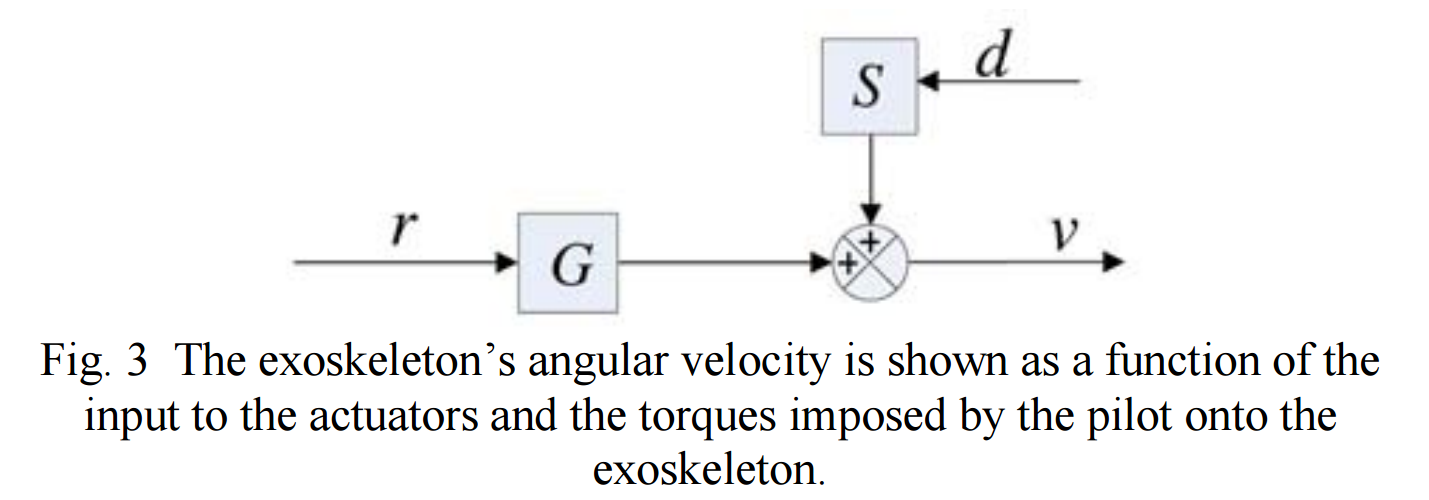
\includegraphics[width=4.0in]{exos/figs/bleex_control_diag_1.png}
\end{figure}

The goal is to maximize sensitivity to $d$ \emph{without direct measurement.}  Sensitivity amplification accomplishes this by creating a feedback loop from a controller, $C$, acting only on exoskeleton variables.  A new sensitivity equation,
\[S_{new} = \frac{v}{d} = \frac{S}{1 + G C} ,\]
is maximized by applying positive feedback.  To achieve a large sensitivity, BLEEX uses $C = (1-\alpha^{-1})G^{-1}$ so that $\alpha$ provides a direct (scalar) amplification factor. A low-pass filter is often added to the $C$ term in order to damp out high frequency dynamics of the exoskeleton, which are not captured in these models.  Note that the controller depends on an inverse dynamic model of the exoskeleton, $G^{-1}$.  Since the model is hybrid, these dynamics switch according to gait phases (single support, double support, stance).  BLEEX detects these transitions using foot sensors.  Assuming the single leg support dynamics are in the form,
\begin{equation}
\mM({\bf\theta})\ddot{{\bf \theta}} + \mC({\bf\theta},\dot{{\bf\theta}}) \dot{{\bf \theta}} + \mV({\bf\theta}) = {\bf T} + {\bf d} ,
\end{equation}
where ${\bf T}$ is a vector of actuator torques, the BLEEX control torque would be
\begin{equation}
{\bf T} = \mV({\bf\theta}) + (1 - \alpha^{-1}) \big [ \mM({\bf\theta})\ddot{{\bf \theta}} + \mC({\bf\theta},\dot{{\bf\theta}}) \dot{{\bf \theta}} \big ] .
\end{equation}
The user must provide the first torque component as the exoskeleton has no actuator acting between the foot and the ground (the system is underactuated).

\begin{figure}[ht]
  \centering
  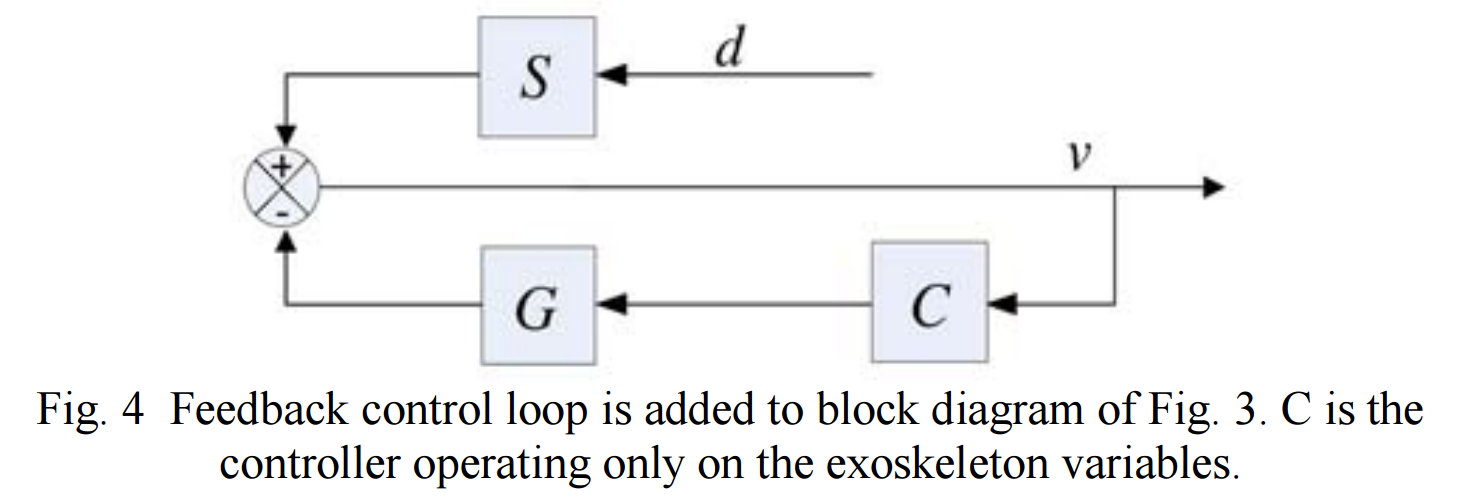
\includegraphics[width=4.0in]{exos/figs/bleex_control_diag_2.png}
\end{figure}

As a note, positive feedback is normally avoided in control design because it amplifies disturbances.  In the case of BLEEX, designers sacrifice disturbance rejection to maximize the response of the suit to its wearer.  Users must therefore take action to stabilize and balance out disturbances.

\begin{figure}[ht]
  \centering
  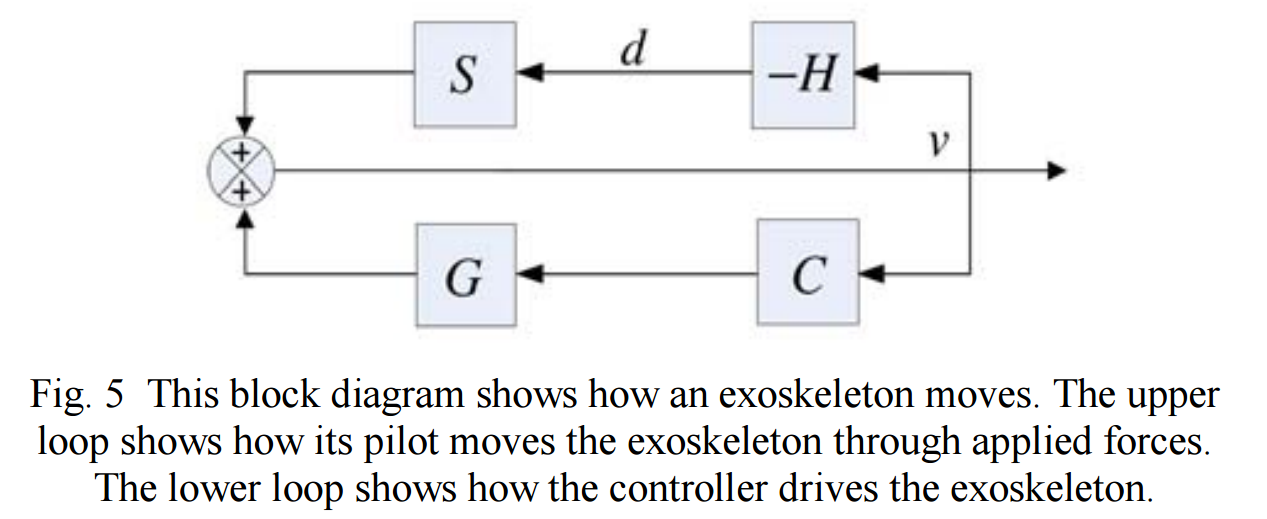
\includegraphics[width=4.0in]{exos/figs/bleex_control_diag_3.png}
\end{figure}

For sensing, BLEEX uses information from \textbf{8 encoders} and \textbf{16 accelerometers} to determine angle, angular velocity, and angular acceleration of eight actuated joints. It includes a \textbf{foot switch and load distribution sensor} at each foot. Eight single axis \textbf{force sensors} provide measurements required to perform low level force control at each actuator. An \textbf{inclinometer} indicates the orientation of the backpack relative to gravity. Using this sensitivity amplification control scheme, BLEEX has achieved successful walking at 1.3 m/s with a 34kg payload \cite{sesitivityAmpPaper2005}.

\subsection{Assessment and Recommendations}

Sensitivity amplification is a current best-in-class control strategy.  The exoskeleton shadows the user and uses exoskeleton data for joint angle, velocity, and acceleration and the exoskeleton model to minimize torques experienced by the human torque.  The process and hardware are relatively simple yet effective.   However, the approach has several significant disadvantages including heavy reliance on an accurate exoskeleton model and the fact that sensitivity amplification will amplify disturbances.  Note that in combat situations this latter point is critical as a sensitivity amplification will amplify forces acting on the suit and the operator will have to re-act to compensate.  The only way to compensate for or resist external forces in this setting is to filter them out, which would be extremely challenging unless additional sensory equipment is provided.  As one possibility, a sensitivity optimization approach may be paired with sEMG data to estimate user intent and provide such a filter.  Note this type of implementation would present its own challenges considering limitations in sensing and calibration of current EMG systems. 

\printbibliography[heading=subbibliography]

The figures in this section were obtained from \cite{sesitivityAmpPaper2005}. Materials presented are based on the references above.

\end{refsection}